\documentclass{juliacon}
\setcounter{page}{1}

\usepackage{amsmath}
\usepackage{footmisc}
\usepackage{etoolbox}
\BeforeBeginEnvironment{lstlisting}{\vspace{-\baselineskip}}
\AfterEndEnvironment{lstlisting}{\vspace{-\baselineskip}}

% \usepackage{todonotes}
% \usepackage[disable]{todonotes}

% \newcommand{\bdv}[2][] {\todo[inline,backgroundcolor=blue!20!white, #1]{(bdv) #2}}
% \newcommand{\ismail}[2][] {\todo[inline,backgroundcolor=red!20!white, #1]{(ismail) #2}}
% \newcommand{\dmitry}[2][] {\todo[inline,backgroundcolor=teal!20!white, #1]{(dmitry) #2}}

\begin{document}
% **************GENERATED FILE, DO NOT EDIT**************

\title{ExponentialFamilyManifolds.jl: Representing exponential families as Riemannian manifolds}

\author[1]{Mykola Lukashchuk}
\author[1]{Dmitry Bagaev}
\author[2]{Albert Podusenko}
\author[2]{{\.{I}}smail {\c{S}en\"{o}z}}
\author[1]{Bert de Vries}

\affil[1]{Department of Electrical Engineering, Eindhoven University of Technology, the Netherlands}
\affil[2]{Lazy Dynamics BV, Eindhoven, the Netherlands}


\keywords{Exponential Family, Julia, Manifold Optimization, Optimization, Probability Distributions}

\hypersetup{
pdftitle = {ExponentialFamilyManifolds.jl: Projecting Probability Distributions onto Exponential Family Members},
pdfsubject = {JuliaCon 2024 Proceedings},
pdfauthor = {Mykola Lukashchuk, Dmitry Bagaev},
pdfkeywords = {Probability Distributions, Optimization, Manifold Optimization, Julia, Exponential Family},
}


\maketitle
\begin{abstract}
\texttt{ExponentialFamilyManifolds.jl} implements exponential family natural parameter spaces as Riemannian manifolds, enabling geometric optimization over probability distributions. The package automatically manages parameter constraints, such as ensuring the positive definiteness of precision matrices for normal distributions. By representing exponential family distributions as manifolds that conform to the \texttt{ManifoldsBase.jl} interface, it allows users to leverage optimization techniques from \texttt{Manopt.jl} for these manifolds. Applications in maximum likelihood estimation and variational inference highlight the package's practical utility.
% while providing advanced optimization techniques by integrating \texttt{ExponentialFamily} with \texttt{Manifolds}. Applications for maximum likelihood estimation and variational inference demonstrate the package's practical utility.
\end{abstract}

\section{Introduction}

Probabilistic inference problems can often be formulated as optimization problems, such as maximum likelihood estimation (MLE) or variational inference (VI) \cite{blei_variational_2017}. In practice, this often involves optimizing over a space of probability distributions to find one that best fits the data (MLE) or approximates a target distribution (VI). Unfortunately, direct optimization over arbitrary probability distributions is intractable. To address these challenges, we often resort to solutions within parametric families, with the exponential family of distributions being a popular choice for its ability to transform inference into convex optimization problems and its natural emergence from maximum entropy principles \cite{wainwright_graphical_2008}. As detailed in \cite[Chapter~3]{wainwright_graphical_2008}, this family not only includes many common distributions like Gaussian, Dirichlet, and Wishart, but also provides a unified mathematical framework for representing graphical models while ensuring distributions maintain maximal uncertainty consistent with observed data. Formally, a distribution is a member of the exponential family if there exists a parameter vector $\eta$ such that its probability density can be written as
\begin{equation*}\label{eq:exponential-family}
p(x|\eta) = h(x)\exp\left(\eta^\top T(x) - A(\eta)\right),
\end{equation*}
where $\eta$ is called the natural parameter. Although this parametrization makes optimization more tractable, challenges remain due to the geometric constraints on the parameter space. For example, the natural parameter vector $\eta$ for a multivariate Normal distribution includes a matrix component proportional to the negative precision matrix.

We present \texttt{ExponentialFamilyManifolds.jl}, a Julia \cite{bezanson2017julia} package that addresses these challenges by implementing the parameter spaces as Riemannian manifolds. By bridging \texttt{ExponentialFamily.jl} \cite{Senoz_ExponentialFamily_jl_2023} with the manifold interface from \texttt{ManifoldsBase.jl} \cite{axen_manifoldsjl_2023} and concrete manifolds from \texttt{Manifolds.jl}, the new package enables geometrically aware optimization techniques to handle parameter constraints automatically using \texttt{Manopt.jl} \cite{bergmann_manoptjl_2022}.

\section{A tour through \texttt{ExponentialFamilyManifolds.jl}}
In this section, we introduce the \texttt{NaturalParametersManifold} interface, the core functionality of our package. We then demonstrate how this interface can be applied to optimization tasks such as maximum likelihood estimation and variational inference.

\subsection{The core interface: \texttt{NaturalParametersManifold}}

A key feature of the core interface \texttt{NaturalParametersManifold} from \texttt{ExponentialFamilyManifolds.jl} is that any point on a manifold—used within \texttt{Manopt.jl}—can also be viewed as an exponential-family distribution. This dual view means we can invoke typical distribution operations (e.g., \texttt{rand} or \texttt{logpdf}) on the same object that supports geometric operations like \texttt{retract}. In other words, we can both \emph{manipulate} a point as part of a manifold-based optimization routine, and use it to \emph{evaluate} functions that treat a point as a distribution for operations like likelihood and sampling.

The \texttt{NaturalParametersManifold} is implemented as a subtype of \texttt{ManifoldsBase.AbstractDecoratorManifold}, defining a generic interface to construct and work with the natural-parameter space of an arbitrary exponential-family distribution. This "decorator" approach allows us to extend the functionality of a base manifold while preserving its core operations. For example, the natural parameters of the Beta distribution form the manifold

\[
\mathcal{M}_{\mathrm{Beta}} \;=\; (-1,\infty) \times (-1,\infty)\,,
\]

which can be represented using \texttt{ProductManifold} from \texttt{ManifoldsBase.jl} together with concrete manifolds from \texttt{Manifolds.jl} through coordinate transformations, which we call \texttt{partition\_point} and \texttt{transform\_back}; the first one takes a natural parameter and transforms it into the corresponding manifold (in the Beta case, shifting it by 1), and the second one is the inverse operation.

\texttt{ExponentialFamilyManifolds.jl} offers an interface to construct \texttt{NaturalParametersManifold} objects \begin{lstlisting}[language=Julia]
M = get_natural_manifold(Beta, ())
\end{lstlisting} The method takes a distribution type, a dimensions tuple (empty for univariate distributions, or e.g., \texttt{(3,)} for 3D multivariate normals), and an optional conditioner. This produces a manifold \texttt{M} on which each point corresponds to valid parameters of the Beta distribution. To obtain a standard \texttt{ExponentialFamilyDistribution} object from a point \texttt{p} on \texttt{M}, we use \texttt{convert(EFD, M, p)}\footnote{\label{foot-efd}Note that to make the listings smaller in place of \texttt{ExponentialFamilyDistribution}, we write \texttt{EFD}.} method. Internally, \texttt{convert} applies \texttt{transform\_back(M, p)} to recover the usual parameter vector before constructing the distribution. An example of this can be seen in Listing~\ref{lst:mle}, where we use \texttt{convert} inside an MLE routine.

\subsection{Using \texttt{ExponentialFamilyManifolds.jl} for Optimization} \label{sec:using_efm}

\texttt{ExponentialFamilyManifolds.jl} transforms distribution-approximation tasks 
(e.g., maximum likelihood estimation or variational inference) into manifold-optimization problems, 
allowing users to focus solely on defining an objective function. 
Listing~\ref{lst:generic_opt} demonstrates a generic workflow for performing gradient-based optimization on a manifold \texttt{M}: 
first, compute the gradient of the objective \texttt{f} using \texttt{ManifoldDiff.jl}, which provides differentials for functions defined on manifolds that implement the \texttt{ManifoldsBase.jl} interface \cite{axen_manifoldsjl_2023}, 
and then execute \texttt{gradient\_descent} from \texttt{Manopt.jl}. 
The \texttt{gradient\_descent} function iteratively applies the \texttt{retract} method to update parameters along the negative gradient direction.
\begin{lstlisting}[language=Julia, caption={Generic manifold-based optimization}, label={lst:generic_opt}]
function optimize(M, f, η_init)
    # compute the Riemannian gradient
    # ... your differentiation backend here
    g(M, η) = ManifoldDiff.gradient(M, f, η, backend)
    return gradient_descent(M, f, g, η_init)
end
\end{lstlisting}
\vspace{1em}

To perform MLE and VI, we only need to define their respective objective functions, the negative log-likelihood for MLE, and the Free Energy for VI, and then use the generic \texttt{optimize} function to perform the inference \footnote{The complete example is implemented in the code at \url{https://github.com/ReactiveBayes/ExponentialFamilyManifolds.jl/blob/paper/paper_example/paper_example.jl}.}. The objective functions for MLE and VI are provided in listings~\ref{lst:mle} and \ref{lst:vi}, respectively \footref{foot-efd}. Figure~\ref{fig:comparisons} shows the results of both approaches. The upper panel demonstrates how MLE and VI produce different approximations to the same target distribution, while the bottom panel compares different families of the approximating distribution.
\vspace{-0.5em}
\begin{lstlisting}[language=Julia, caption={Objective functions for MLE}, label={lst:mle}]
function f_mle(M, η, samples)
    dist = convert(EFD, M, η)
    return -mean(logpdf(dist, s) for s in samples)
end
\end{lstlisting}
\vspace{-0.5em}
\begin{lstlisting}[language=Julia, caption={Objective functions for VI}, label={lst:vi}]
function f_vi(M, η, t, size)
    q = convert(EFD, M, η)
    samples = rand(MersenneTwister(22), q, size)
    diff(s) = logpdf(t, s) - logpdf(q, s)
    return -mean(diff, samples)
end
\end{lstlisting}
\vspace{1em}
The \texttt{optimize} (the Listing \ref{lst:generic_opt}) function demonstrates how gradient descent can be implemented using the \texttt{NaturalParametersManifold} interface. Additionally, the approach can be easily adapted to use the natural gradient \cite{amari_natural_1998} by incorporating the Fisher information into the gradient computations, as shown in Listing~\ref{lst:natgrad}.

\begin{lstlisting}[language=Julia, label={lst:natgrad}, caption={Computing the natural gradient with \texttt{ForwardDiff.jl} \cite{revels_forward-mode_2016}}]
function natural_gradient(M, p, f, grad)
    q = convert(EFD, M, p)
    F = fisherinformation(q)
    grad = ForwardDiff.gradient(
        x -> f(M, p), p
    )
    return F \ grad
end
\end{lstlisting}

% \dmitry{Reads confusing. What are these \textit{geometric aspects}? Have they been defined?}

% \section{Acknowledgements}

\begin{figure}[tb]
   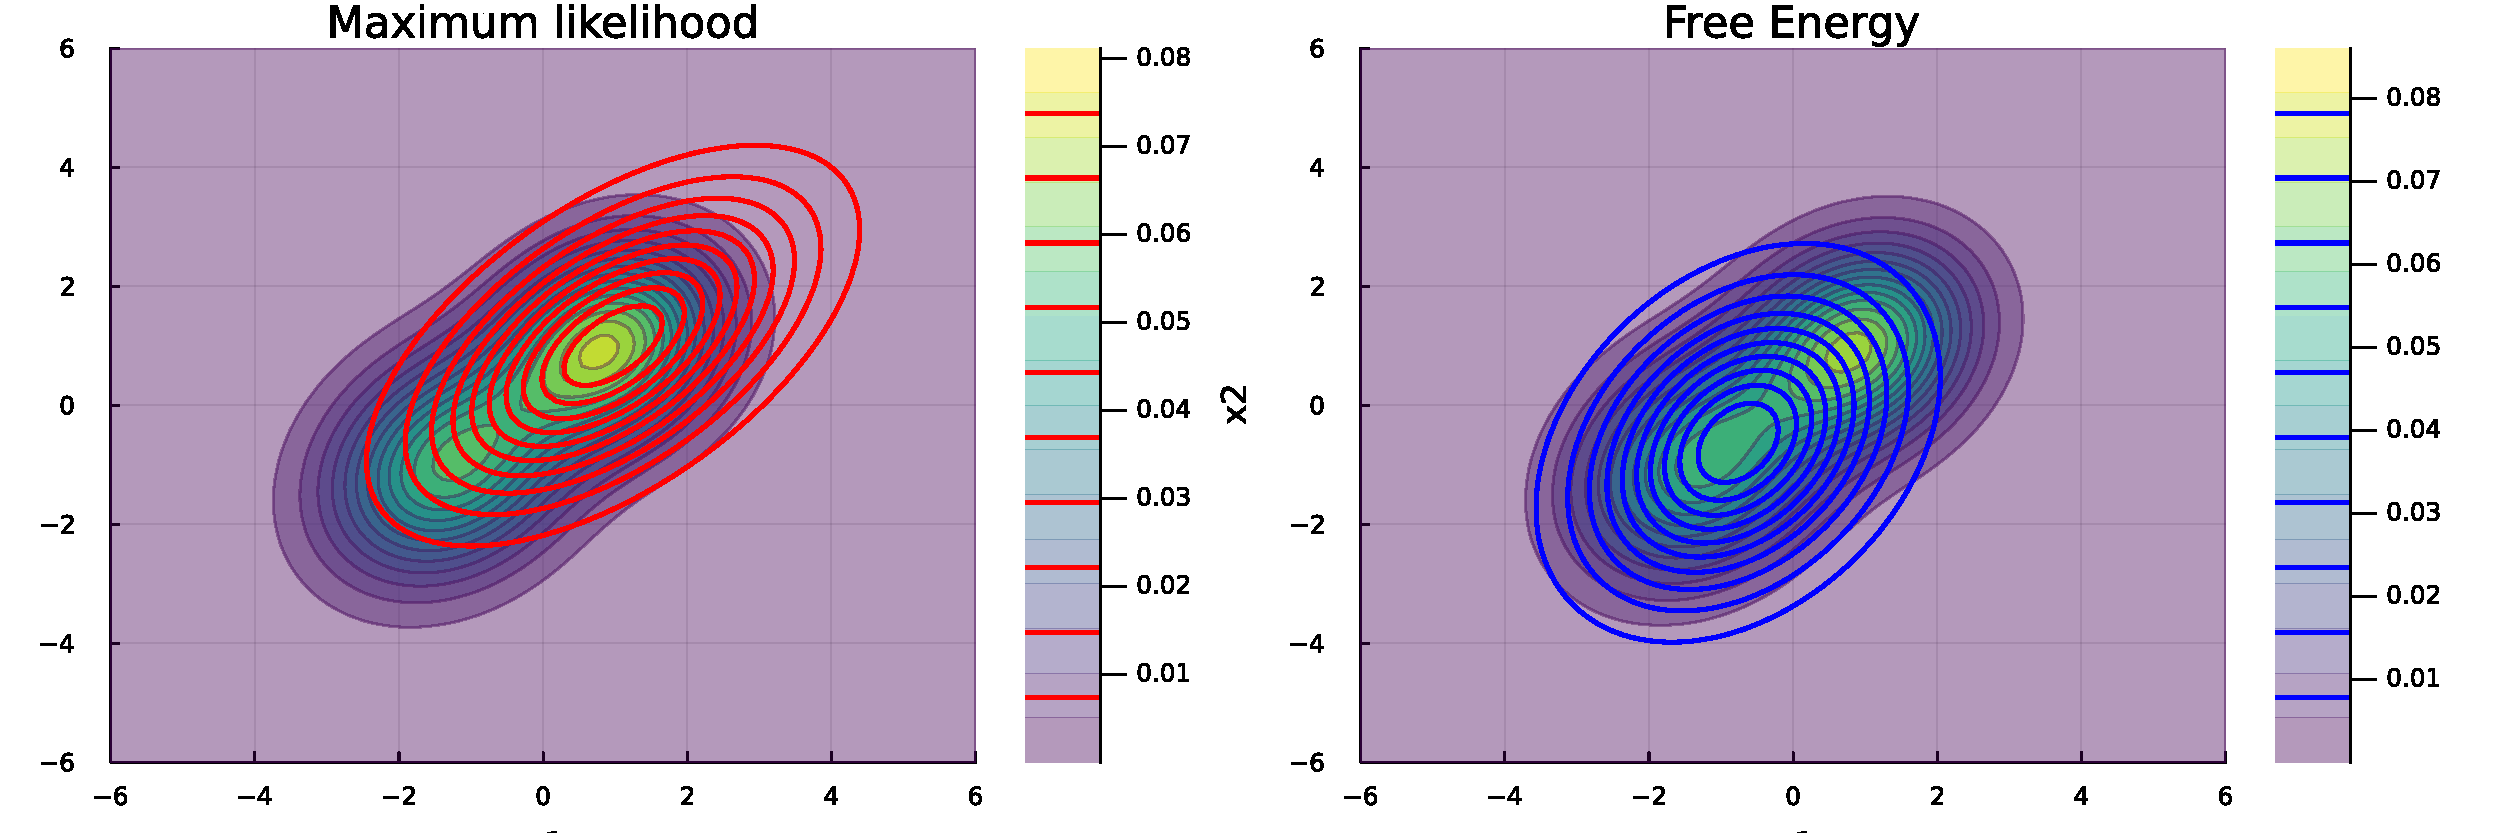
\includegraphics[width=0.48\textwidth]{plots/comparison1.pdf}
   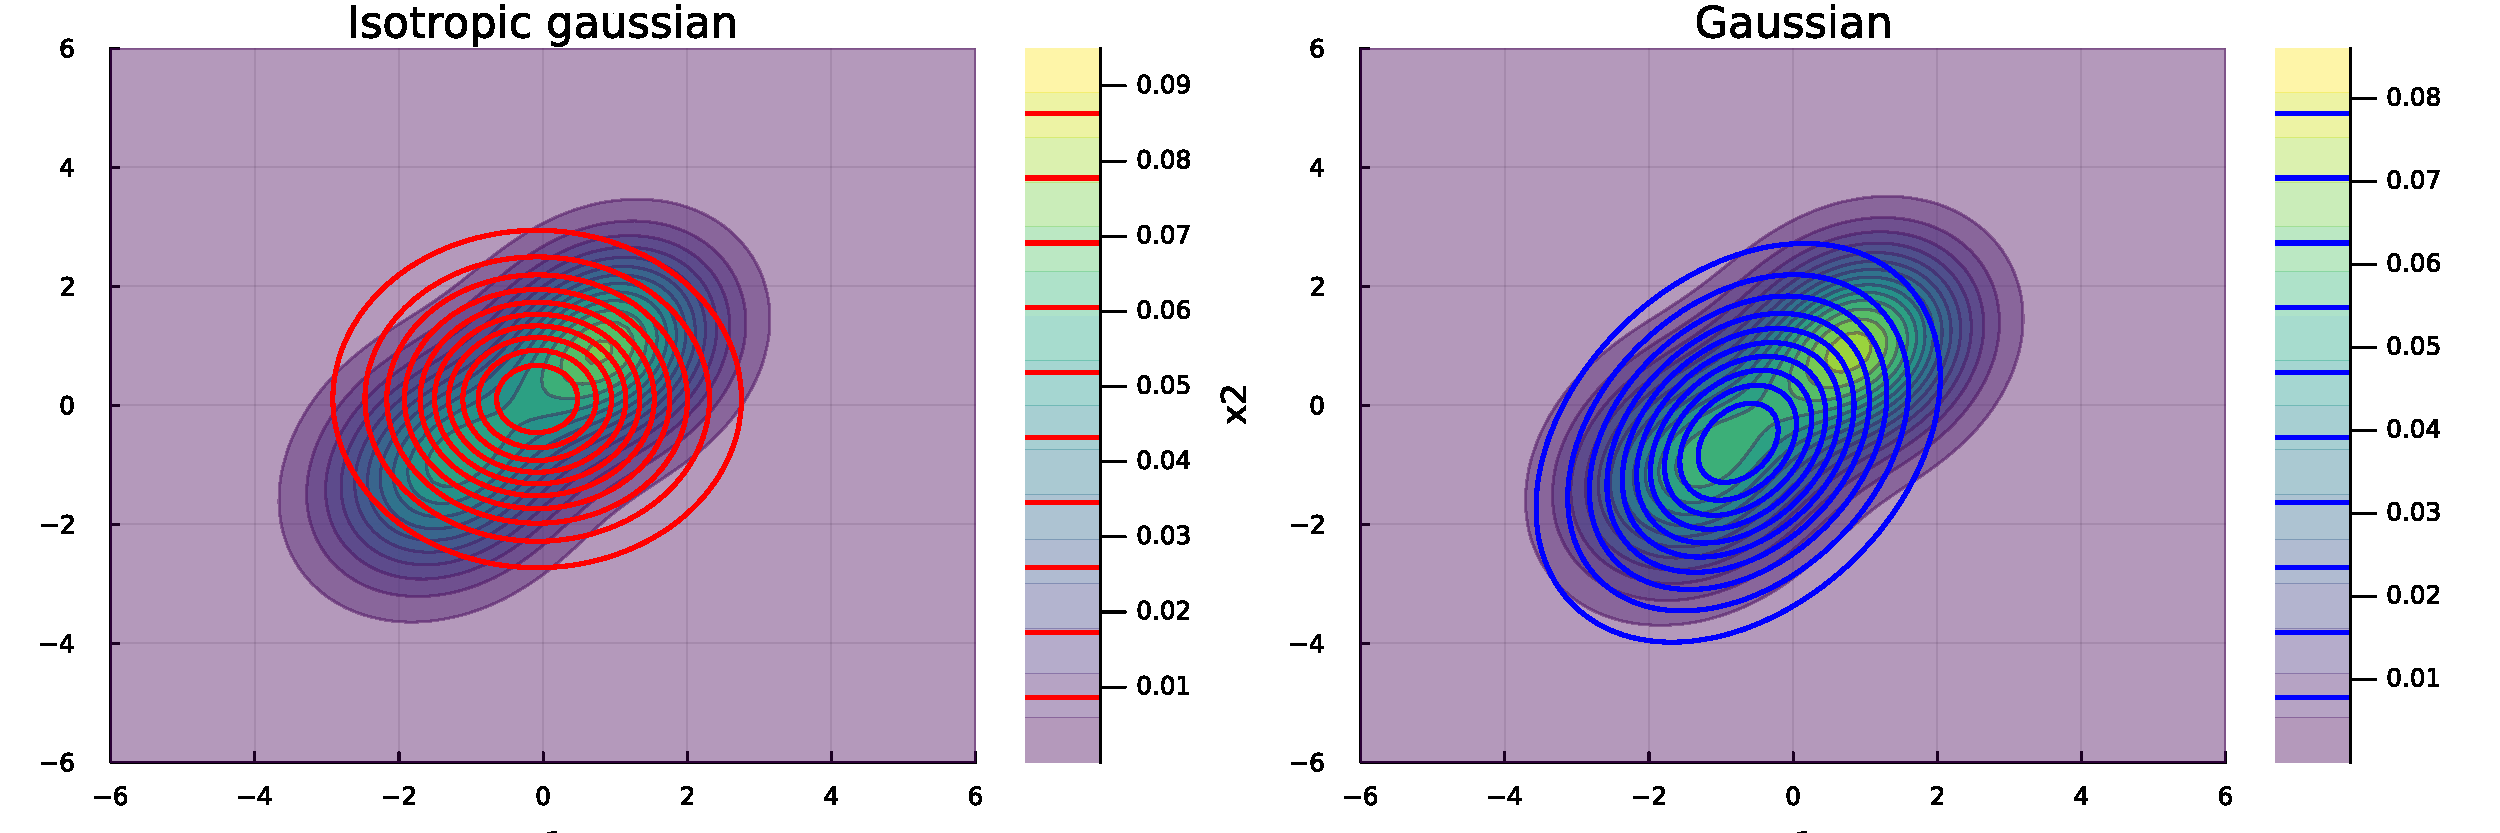
\includegraphics[width=0.48\textwidth]{plots/comparison2.pdf}
   \caption{\textbf{Top:} MLE (red) vs. VI (blue) approximations of a target distribution (shown in the background): a mixture of two Gaussian distributions with different means and covariances. While MLE showed covering behavior towards the target density, VI demonstrated a mode-seeking behavior. \textbf{Bottom:} Isotropic (red) vs.\ full-covariance (blue) Gaussian approximations using Free Energy objective for both, showing the trade-off between computational efficiency and approximation quality - Isotropic Gaussian approximations are fast to obtain, but less flexible than full-covariance Gaussians.}
   \label{fig:comparisons}
\end{figure}

\section{Future work}
While most of the distributions in this package use product manifold geometry, the Fisher-Rao metric~\cite{amari_natural_1998} provides a more suitable geometry for exponential families, potentially leading to more robust optimization (see Listing~\ref{lst:natgrad}). Additionally, extending the package to support mixture families of exponential family distributions could enhance its capabilities since, for example, mixture models can better capture multiple modes in VI.


\bibliography{ref}
\bibliographystyle{juliacon}

\end{document}
